\subsubsection{Time schedule}
To be able to plan our time efficiently, we had to find out how much time we had at our disposal. Our way of doing this was to create a custom spreadsheet, containing all the dates until the final deadline. For each date a field for each group member was made, wherein the available time span for that person was entered. This way it was easy for us to get an overview of when we all were available. This helped us a lot in planning our meetings.

Generally, we decided, that if three or more group-members were available, a meeting would be planned. We would rather plan too many meetings and be done with everything early, than plan the exact hours needed to complete all the backlog items and risk time pressure due to unforeseen tasks or delays.

From the first part of the project we had learned that all-nighters - that is, a meeting continuing until the next morning - were effective ways to get a lot of work done, even though the productivity decreased over night. With this experience we converted as many pairs of subsequent days into all-nighters as we deemed it possible (see figure \ref{fig:time_schedule}).

\begin{figure}[H]
  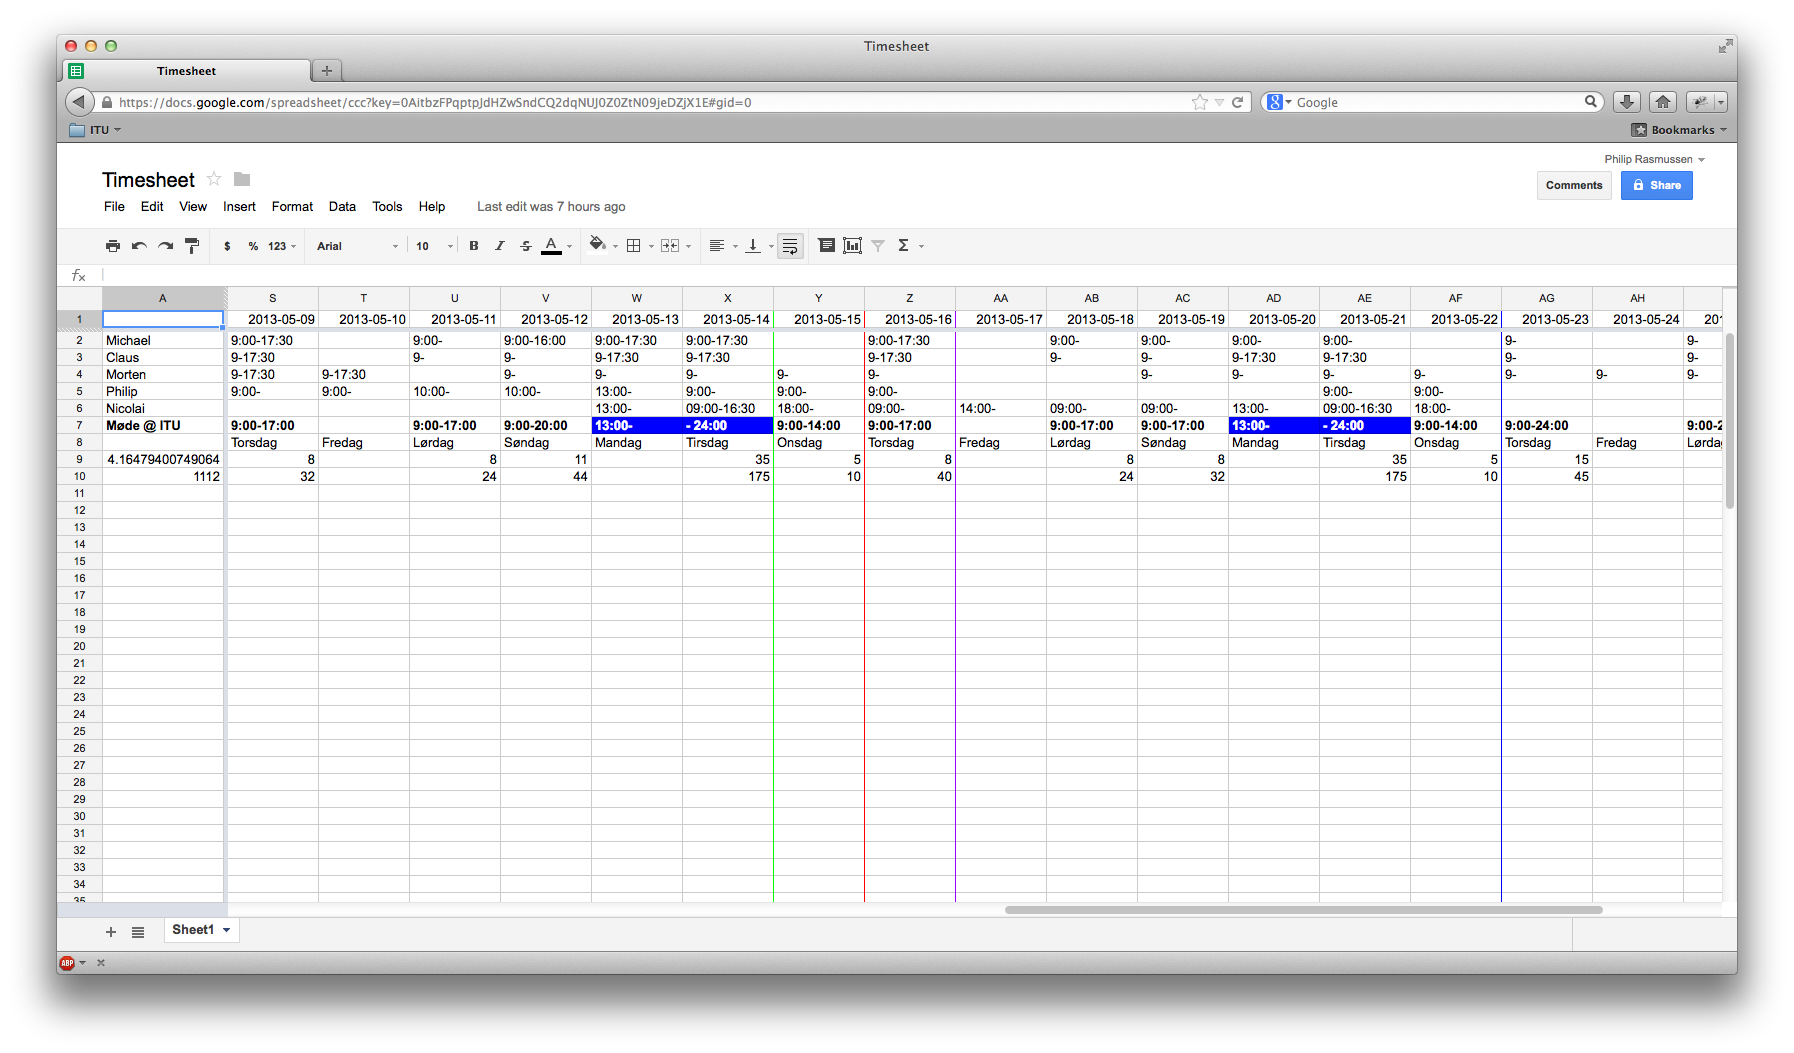
\includegraphics[width=\textwidth]{illustrations/timeSheet}
  \caption{Time schedule}
  \label{fig:time_schedule}
\end{figure}

\cref{time schedule} shows our custom spreadsheet using our custom method. We have had great benefit from doing it this way, as planning group meetings was instantaneous without too much discussion back and forth. The dates with bold time spans indicate days with meetings. The double fields with blue background indicate planned all-nighters.